\documentclass[11pt,a4paper]{article}
\usepackage[utf8]{inputenc}
\usepackage[margin=0.85in]{geometry}
\usepackage{graphicx}
\usepackage{hyperref}
\usepackage{xcolor}

\begin{document}
\noindent\textbf{\Large Tech Nation Visa - Exceptional Promise}\\
\noindent\textbf{Criteria:} Optional Criteria 4 (Academic Contributions through Research)\\
\noindent\textbf{Applicant:} Odeyemi Olusegun Israel\\
\rule{\textwidth}{0.4pt}

\vspace{0.1cm}
\begin{center}
    \textbf{\Large Evidence 4: Academic Publications \& Global Research Impact}
\end{center}
\vspace{0.1cm}

\section*{1. Executive Summary}
\textbf{I wrote and published four research papers} without institutional affiliation, co-authors, or promotion budget on TechRxiv (the IEEE engineering preprint platform) and Zenodo (a CERN-hosted open-access research archive). In under ten weeks they recorded \textbf{365 views and 210 downloads}.

Three were independently selected as required reading for an accredited postgraduate course by a \textbf{Top 2\% World Scientist} (Stanford University annual citation impact ranking), without any prior contact with me. The course evidence is documented separately in the OC4 CPE 604 Addendum.

\section*{2. The AMTTP Infrastructure Paper (TechRxiv)}
\textbf{Published:} 27 February 2026 \quad $\vert$ \quad \textbf{Metrics:} 230 Views, 153 Downloads (as of 5 May 2026)\\
\textbf{DOI:} \texttt{10.36227/techrxiv.177220113.33816607/v1}\\
The first paper, introducing the AMTTP system design to the academic community --- specifically how the blockchain enforcement layer and the AI fraud-detection engine are connected. It recorded 230 views and 153 downloads in roughly ten weeks, with no institutional promotion.

\vspace{0.05cm}
\begin{center}
    \fbox{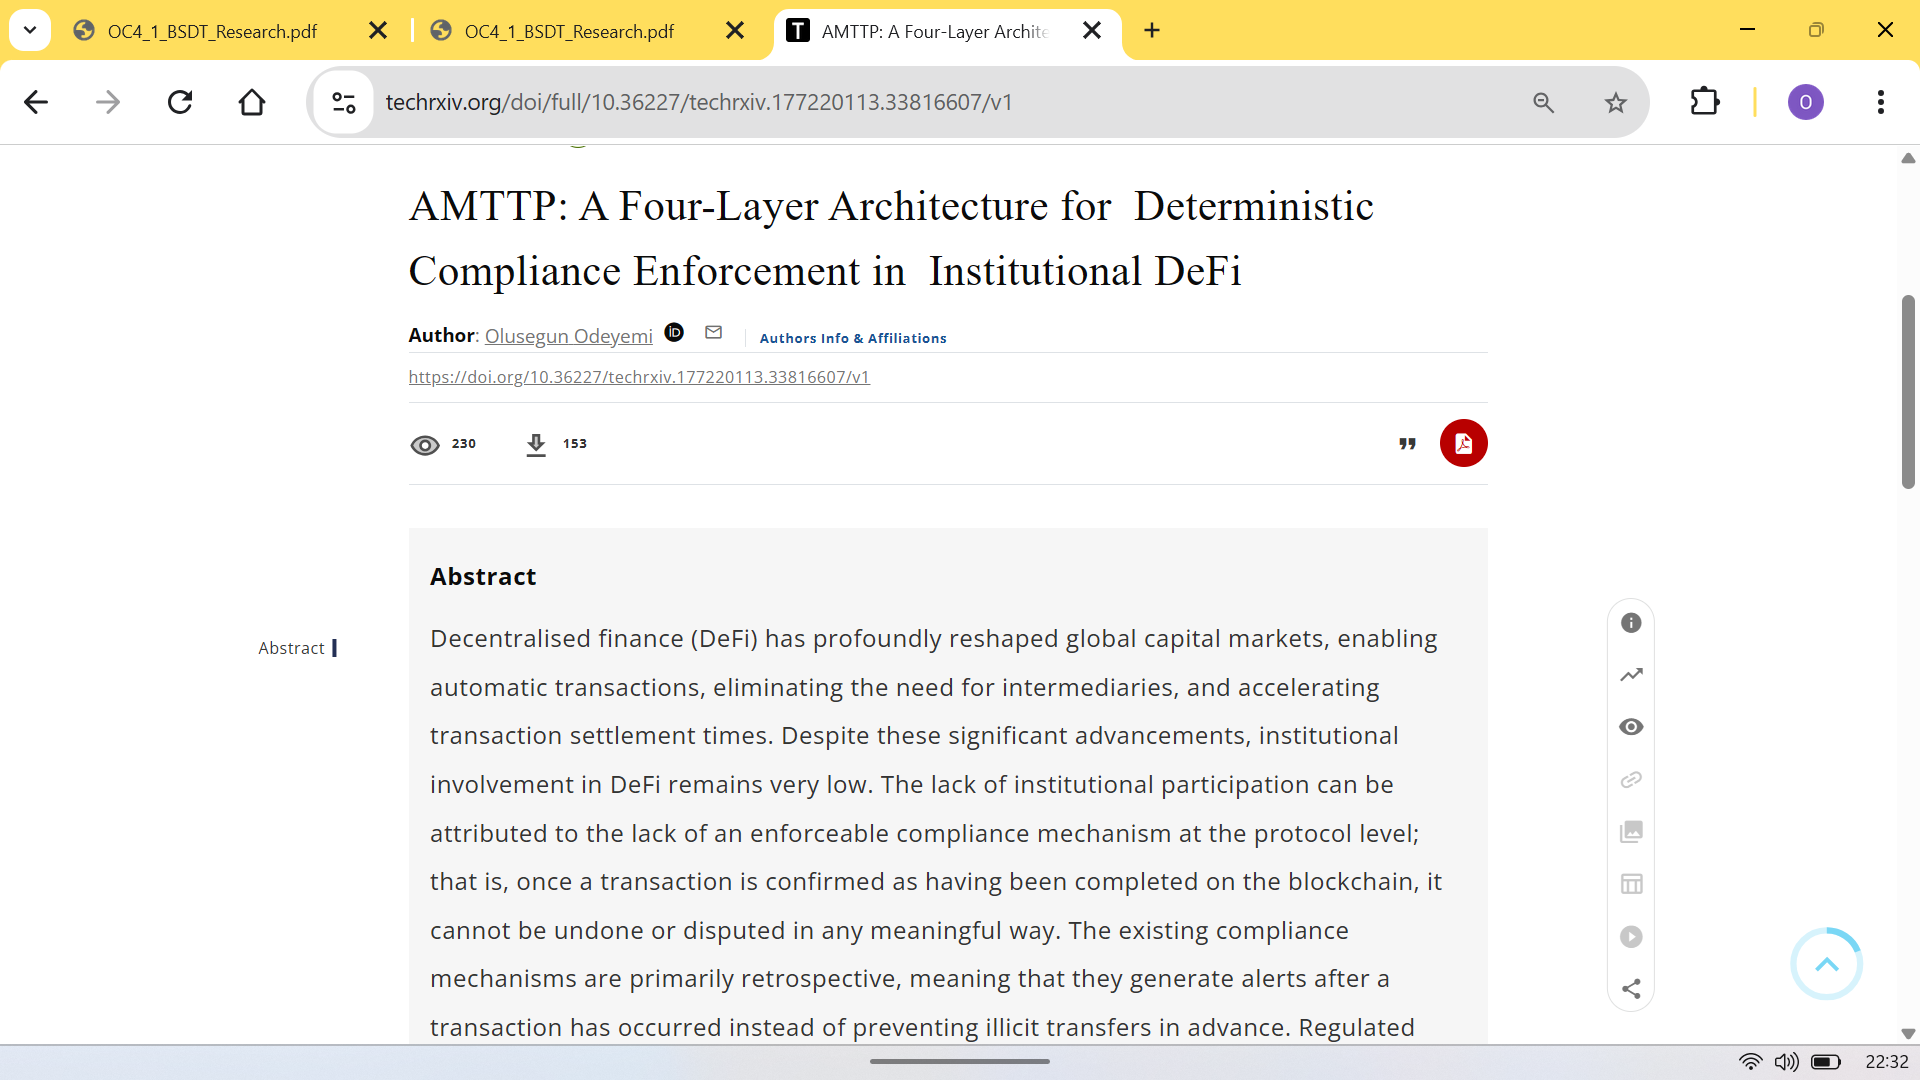
\includegraphics[width=0.78\textwidth]{images/techrxiv_amttp.png}}
\end{center}
\vspace{0.02cm}
\textit{Figure 1: TechRxiv analytics --- 230 views, 153 downloads; 10 weeks, no institutional promotion.}

\section*{3. Blind-Spot Decomposition Theory --- BSDT (Zenodo)}
\textbf{Published:} 5 March 2026 \quad $\vert$ \quad \textbf{Metrics:} 135 Views, 57 Downloads (as of 5 May 2026)\\
\textbf{DOI:} \texttt{10.5281/zenodo.18870590}\\
The theoretical framework paper: its four-channel decomposition, mathematical derivations, cross-domain validation results, and working code implementation are detailed in OC4-1. It recorded 135 views and 57 downloads on Zenodo, confirming independent academic interest.

\vspace{0.05cm}
\begin{center}
    \fbox{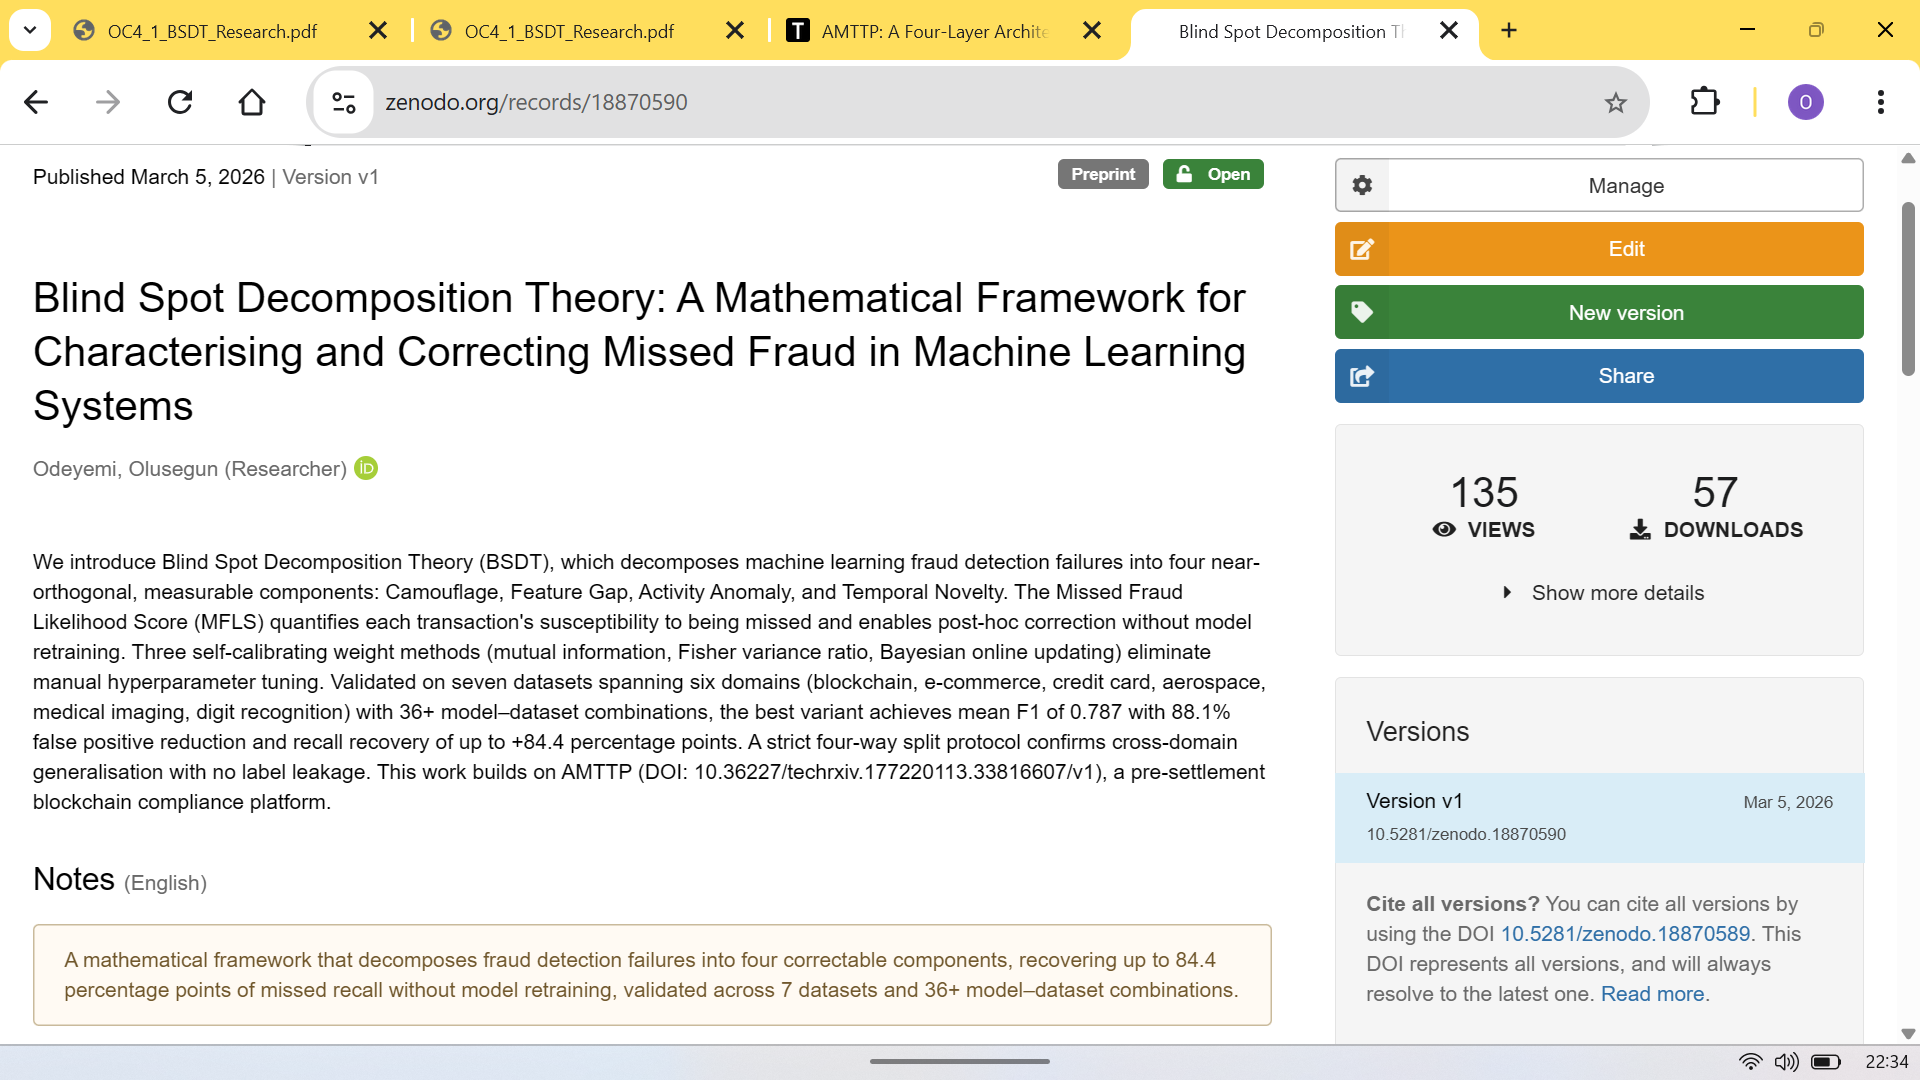
\includegraphics[width=0.78\textwidth]{images/zenodo_bsdt.png}}
\end{center}
\vspace{0.02cm}
\textit{Figure 2: Zenodo analytics --- 135 views, 57 downloads for the BSDT paper. Combined primary papers: 365 views, 210 downloads.}

\section*{4. Blind-Spot Decomposition and the Geometry of System Collapse (Zenodo)}
\textbf{Published:} 16 March 2026 \quad $\vert$ \quad \textbf{DOI:} \texttt{10.5281/zenodo.19038783}\\
This paper extends BSDT using topology and control theory, testing whether the same framework detects instability beyond financial fraud. It was applied to three independent crisis datasets (2008 US banking crisis, Terra/Luna collapse, 2021 Texas power-grid failure) without retraining; quantitative results are in OC4-1. This is generalisable mathematical theory, not product-specific implementation.

\vspace{0.05cm}
\begin{center}
    \fbox{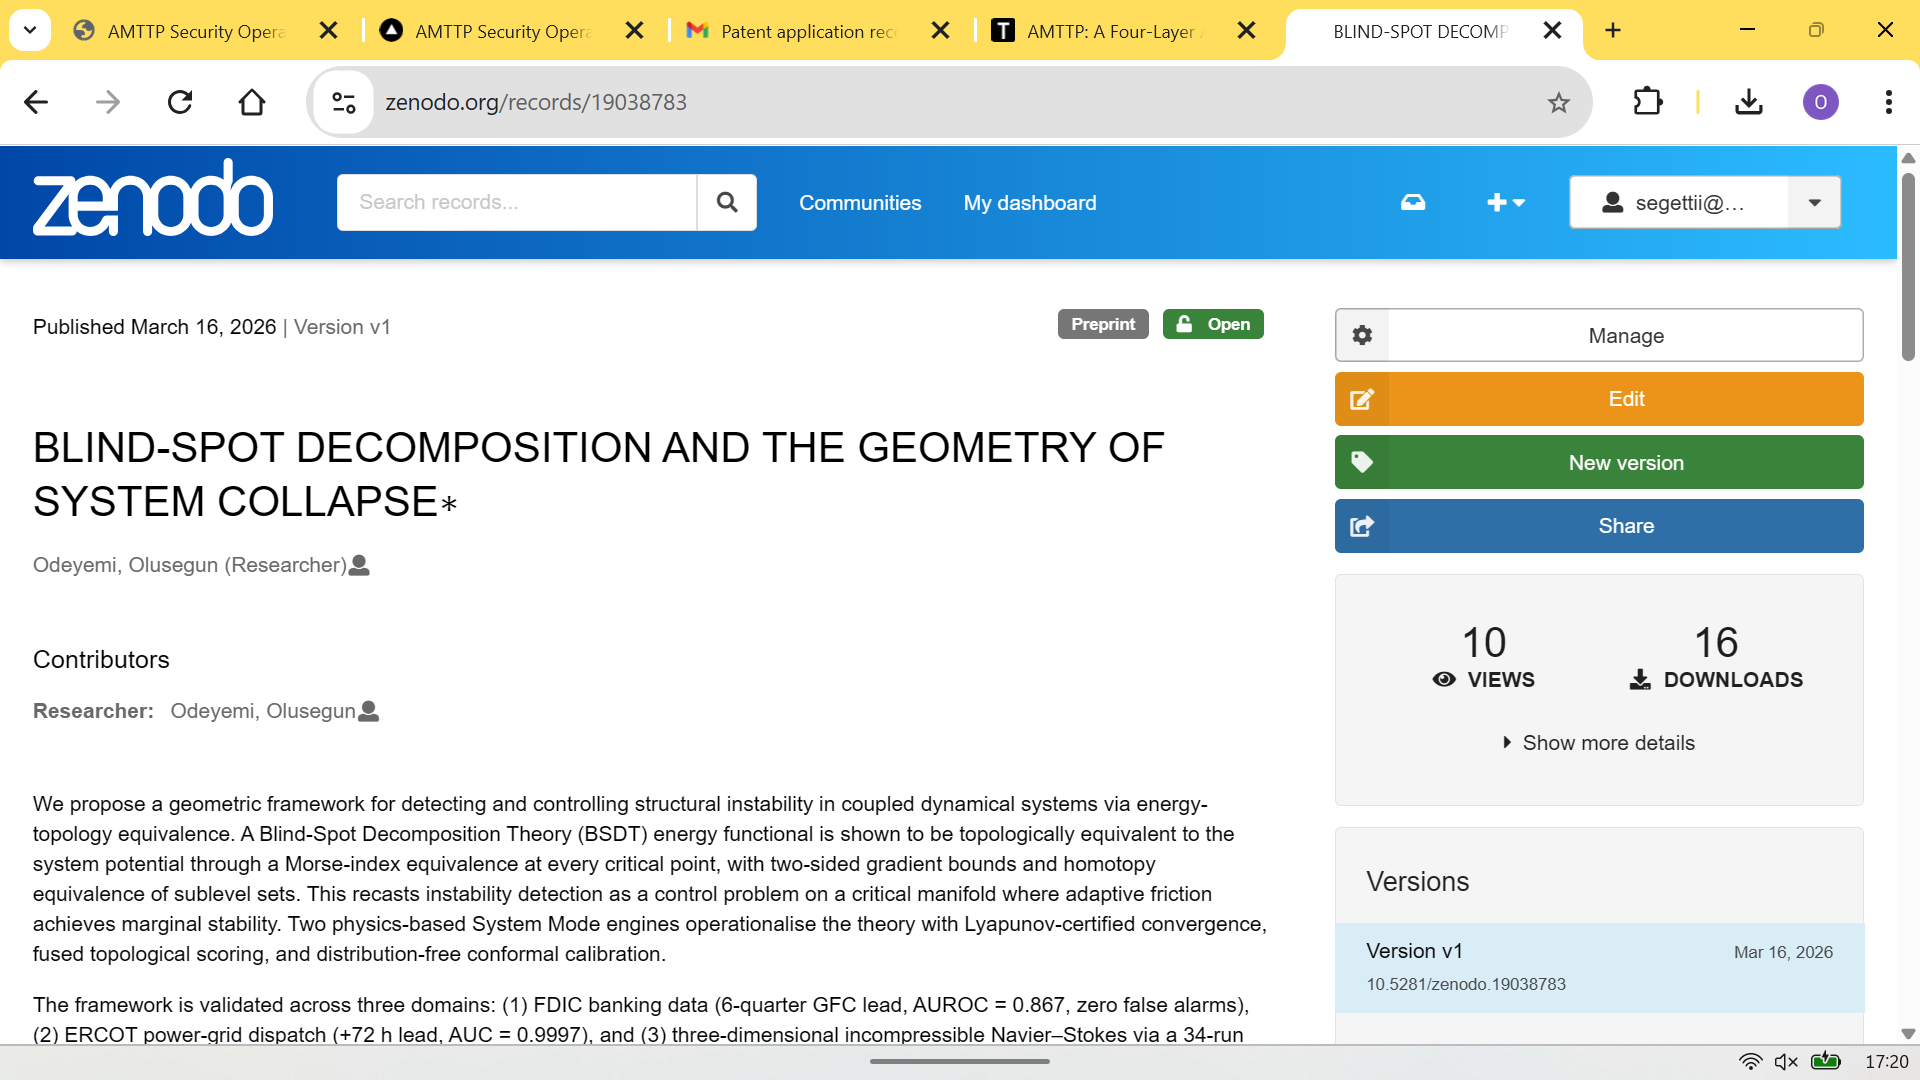
\includegraphics[width=0.78\textwidth]{images/zenodo_geometry.png}}
\end{center}
\vspace{0.02cm}
\textit{Figure 3: Zenodo --- Geometry of System Collapse. Three crisis datasets, no retraining. AUROC 0.9997 on ERCOT.}

\section*{5. Universal Deviation Principle (UDP)}
\textbf{Published:} 15 March 2026 \quad $\vert$ \quad \textbf{Version DOI:} \texttt{10.5281/zenodo.19037688}\\
The fourth paper extends BSDT into a fully general anomaly-detection framework, defining 14 composable operations from five branches of mathematics and formally proving six theoretical guarantees, including reliability with small data samples. It completes the research progression: from AMTTP (applied engineering system), to BSDT (mathematical framework), to UDP (foundational anomaly-detection theory).

\vspace{0.05cm}
\begin{center}
\fbox{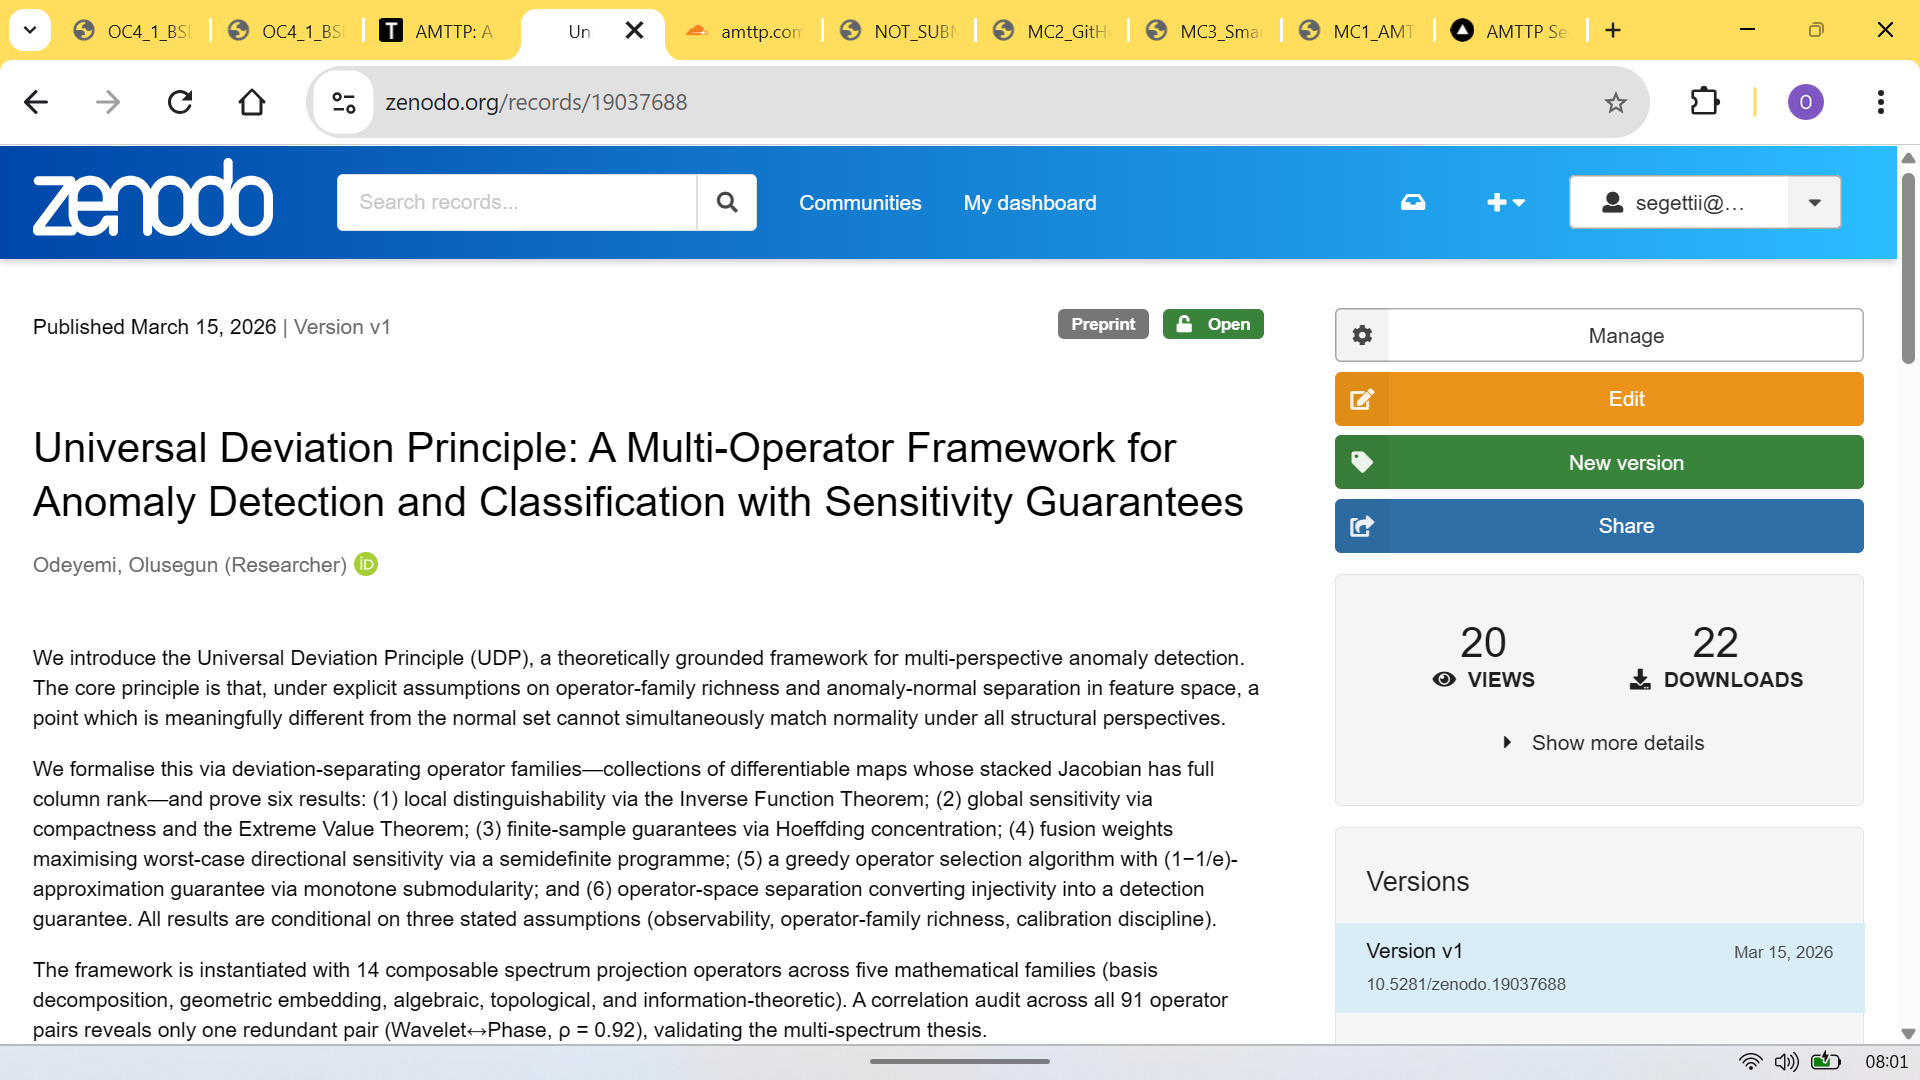
\includegraphics[width=0.62\textwidth]{images/zenodo_udp.png}}
\end{center}
\vspace{0.02cm}
\textit{Figure 4: Zenodo --- UDP paper (20 views, 22 downloads). Evidences continued theoretical output.}

\section*{6. External Academic Recognition}
Both endorsements were unsolicited.

\textbf{Prof.\ A.\,S.\,O.\ Ogunjuyigbe} (Professor of Electrical and Electronic Engineering, Provost of the Postgraduate College, University of Ibadan) independently confirmed that the 72-hour ERCOT advance warning identifies the same precursors documented in the official FERC/NERC post-incident investigation. He judged the work ``\textit{highly significant.}'' An engineering professor with no prior knowledge of my research reached the same conclusion as a federal regulatory body.

\textbf{Dr Sunday Adeola Ajagbe} (Top 2\% of World Scientists 2025, Stanford University; Senior Lecturer, Abiola Ajimobi Technical University; Research Associate, University of Zululand) adopted three of my papers into \textbf{CPE 604} as required postgraduate reading and describes the work as ``\textit{exceptional promise in digital technology.}'' Full course evidence --- lecture slides, signed reference letter --- is in the OC4 CPE 604 Addendum.

\end{document}